\section{Business Model}
%Describe the most important elements in the canvas model for your idea
\begin{figure}
	\centering
	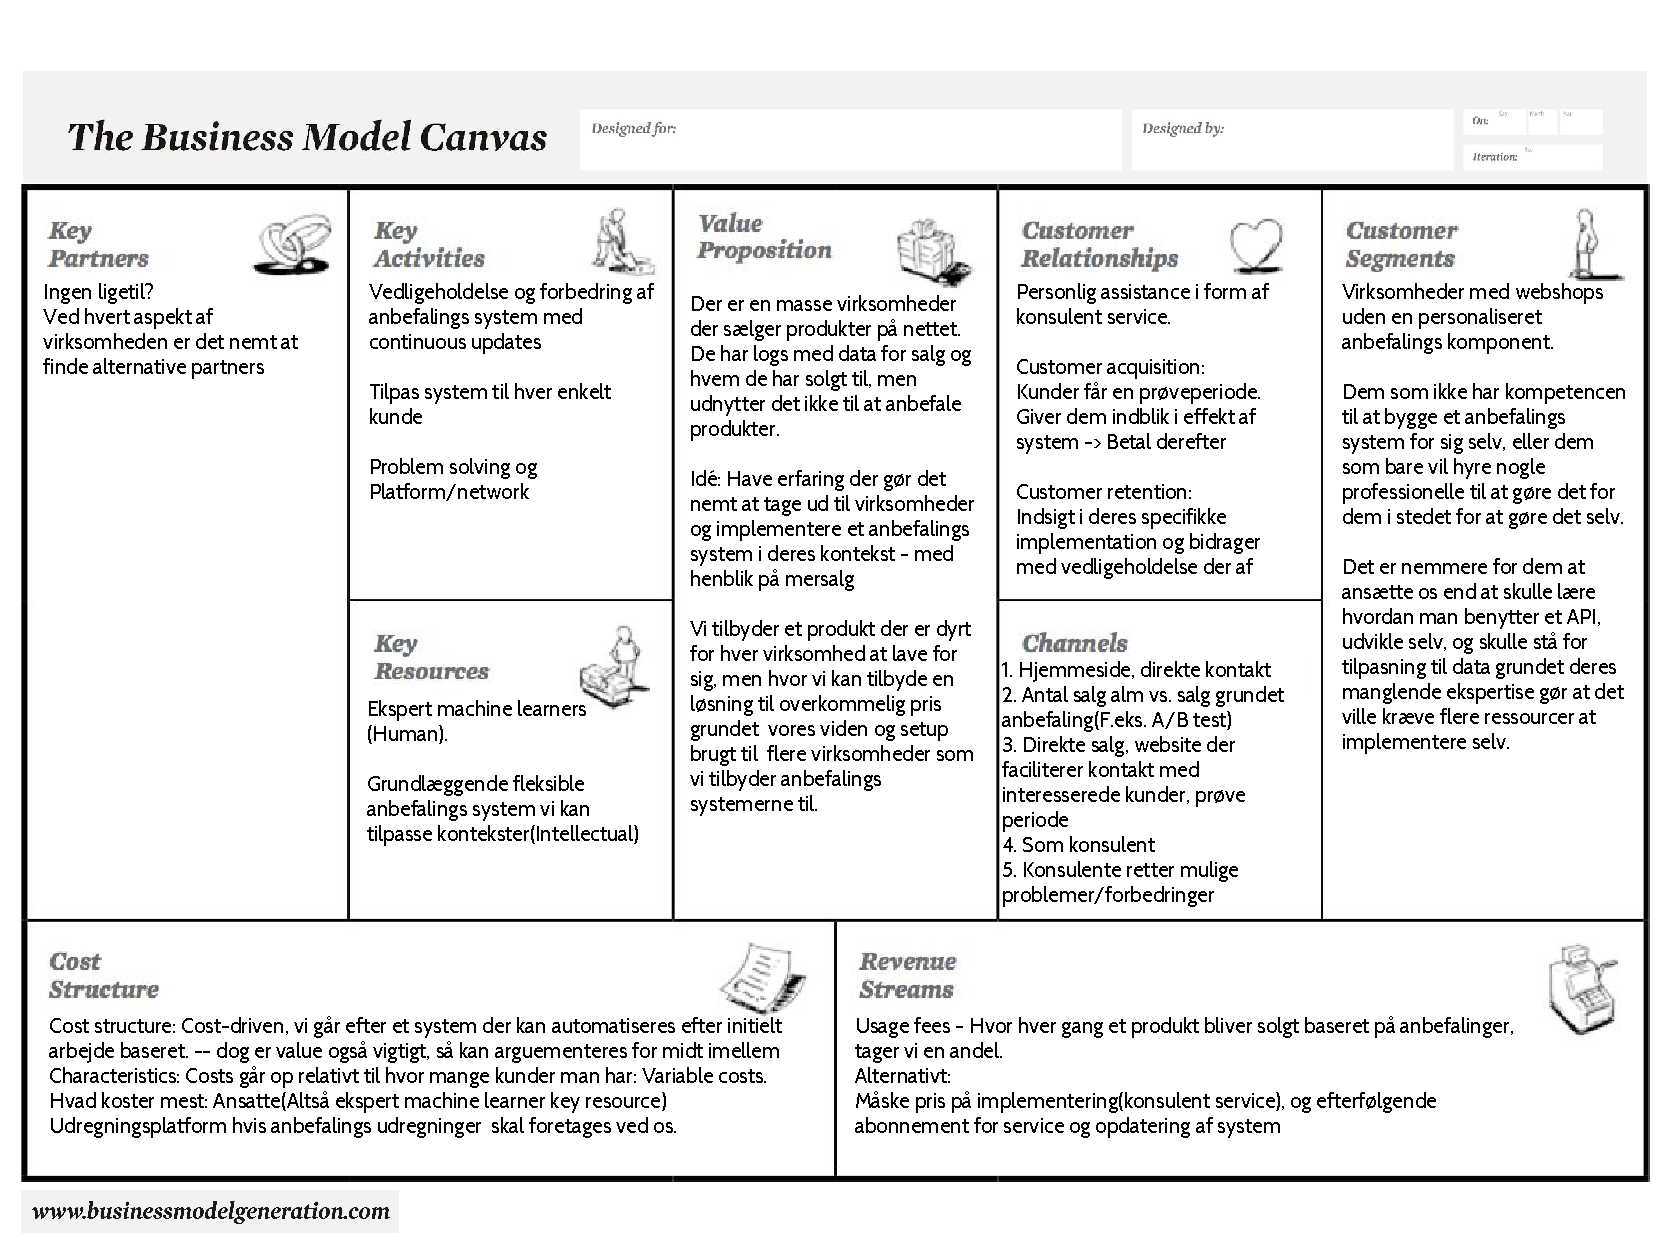
\includegraphics[width = 1.5\textwidth, angle=90]{figures/business-model-canvas}
	\caption{The Business Model Canvas for our Business Idea}
	\label{fig:BusinessModelCanvas}
\end{figure}

%    Describe your team under KR (key resources) - describe your technological expertise
The teams technological expertise lies within Machine Learning, which is where the overall idea comes from, given that product recommendation lies within the domain of machine Learning.

%    Characterize and discuss your VP (value proposition) and other relevant canvas elements using concepts from The software start-up chapter in the course notes (pages 40-55) and the e-Entrepreneurship chapter (pages 57-68)
In order to get an insight into the characteristics of the canvas elements, we answer a series of questions. 
The questions are from \citep[pg. 40-55]{book:jrose}.
The reason we need to answer these questions is because we see ourselves as arbitrageurs.
The arbitrageur exploits market inefficiencies, as there is very few companies that provide e-commerce solutions for local businesses. 
The other companies are typically too expensive for the small firms, and we strive to exploit this.
We exploit it by providing an customised and low-cost alternative.

\begin{description}[style=nextline]
	\item[Do  you  want  to  be  mainly  a  products  company  or  a  services  (consultancy)  company?] We see the product as SaaS(Software as a Service), with some additional optional consultancy work to customise the recommender solution to the webshops. For that reason it is a service company, where we have one core product.
	\item[Do  you  want  to  sell  to  individuals  or  enterprises,  or  to  mass  or  niche  markets?] The target audience of our product is enterprise companies and towards mass markets, as the product can be applied to virtually any webshop.
	\item[How  horizontal  (broad)  or  vertical  (specialized)  is  your  product  or  service?] Our service is vertical because of the scope of the business model. We have a very specialised product, the recommender system service, which we specialise in and strive to continuously improve.
	\item[Can  you  generate  a  recurring  revenue  stream  to  endure  in  good  times  and  bad?] Yes, since it is SaaS. In that way the customers pay a subscription fee to keep using the service.
	\item[Will  you  target  mainstream  customers,  or  do  you  have  a  plan  to  avoid  "the  chasm" - the gap between early adopters (the  rather  few  customers  with  specialised  interests  who  buy technically-innovative products),  and  the  early  majority  (the  many  customers  who  want  to buy  a  product  that  is  technically  sophisticated, but  also  established  and  popular)?] We target mainstream customers, and have no plans on targeting the early adopters or early majority types. In that way, we assume that the mainstream customers do not have the technical abilities to create their own recommender systems or want to invest their resources on developing their own. We think is a reasonable assumption due to the high lack of people with machine learning skills in Denmark.
	\item[Do  you  hope  to  be  a  leader  (a  company  that  is  an  innovator),  follower  (on  that basis  its products  on  established  technologies),  or  complementor  (a  company  that  provides additional  software  and  services  to  an  established  platform)?] We see ourselves as a complementor as we provide additional services that can improve the income of customers' webshop sales.
	\item[What  kind  of  character  (culture,  image,  brand,  working  environment)  do  you  want  your company  to  have?] We want our company to have a professional culture with an image that show that we are a disciplined company with high quality products and services.
\end{description}
Looking at the software business model, \citep[pg. 43]{book:jrose}, our company has a fairly high degree of involvement with the customers relationships, as we are consultants that can help businesses implement our solution. 
Additionally, the homogeneity of the product is also high, given that we want a standard backend that can be utilized in many different shops. 
As such we fit the ‘applied formats’, which means that we are offering a customizable solution based on a standard platform. One could also argue that it is software tailoring, since we customise the recommender system to the customers need, but what is tailored for each customer is only the parameters, e.g. their sales data and how to use it.

If we look at the software revenue generation model it can be characterised as SaaS.
We do, however, have a slight twist, since we use a free trial period.
Once the trial period is over though, the customer will be used to the increased sales that our system provides and sees no other option than paying us for a continuous use of the service.
In that way we can say that we use the bait \& hook pattern.

%    Discuss your canvas model. For example describe how it supports the implementation of your idea. Is it likely to change over time?
%    You may discuss pattern considerations (e.g. FREE or Open Business Models) using relevant concepts from the course notes
%    You may discuss your design approach (e.g. Customer Insights or Scenarios) using relevant concepts from the course notes
%    You may describe strategy concerns (e.g. Business Model Environment, Evaluation or Blue Ocean) using relevant concepts from the course notes

The canvas model gives a good representation of how we can bring our idea to life.
It describes the value proposition well, which is what part of the canvas that is least likely to change. 
However, as we get more customers, the solution may become less customised to each firm we provide a service to, and more of a standardised solution.

One could imagine that depending on the customers we are in contact with, the revenue stream may change. 
An alternative to the subscription based solution is to make an agreement with the company that we gain a part of the profit from the increased sales that the recommender system provides.
Such a change may be interesting for webshops we believe have an extreme growth potential.

For the other parts of the business canvas model, we cannot at this point in time imagine what may change. 
However, one of the advantages of the business canvas model is that it gives a short outline of the business model that can be changed if necessary as we experience change in our entrepreneurial process.

\subsection{Storytelling}
To gain a better outlook of the business idea, and to illustrate how we utilise the bait \& hook pattern, we drew a storyboard, which can be seen in Figure \cref{fig:drawing}.

\begin{figure}
	\centering
	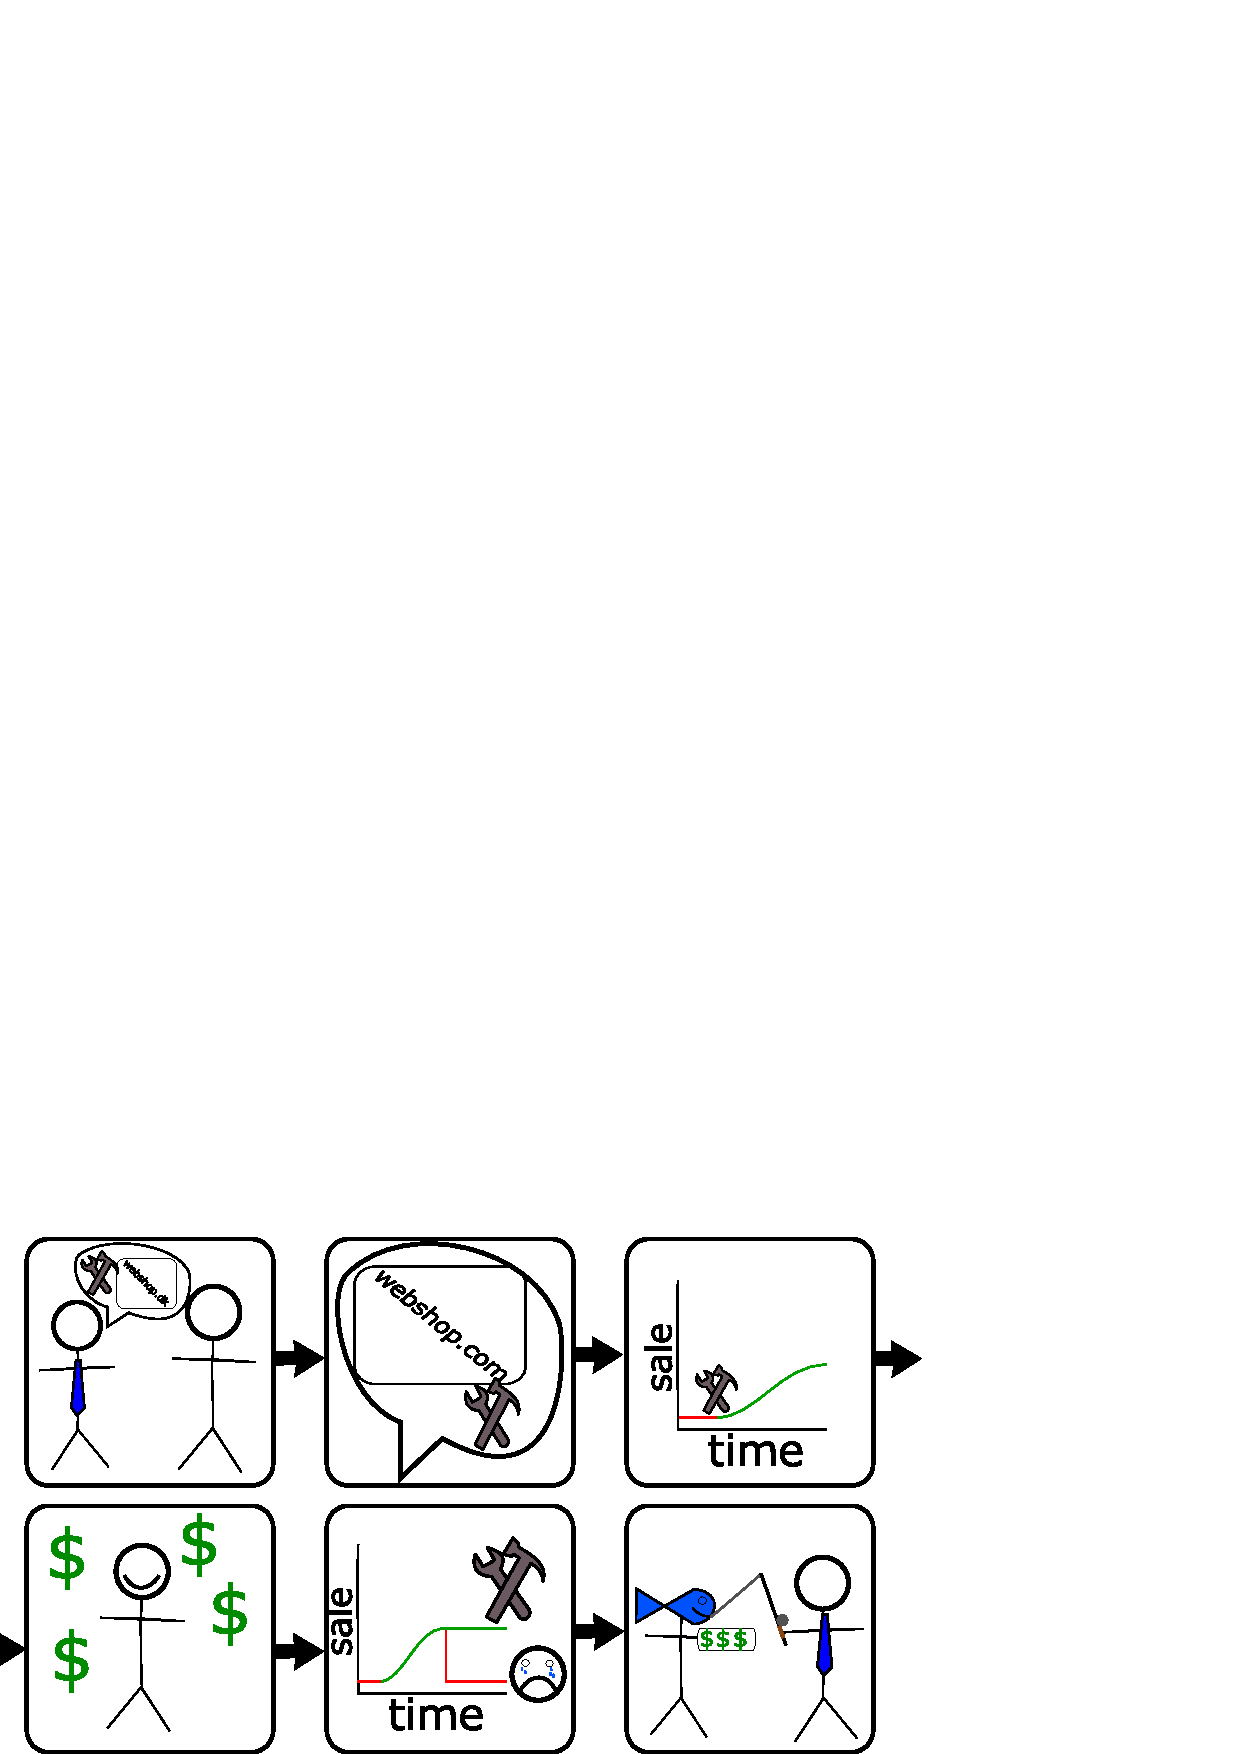
\includegraphics[width=0.7\linewidth]{figures/drawing}
	\caption{Story board of how we use the bait \& hook pattern.}
	\label{fig:drawing}
\end{figure}
 
 On frame one and two we introduce our recommender system solution to the customer who owns a webshop.
 Frame 3 and 4 shows how the customer becomes happy since our solution increased his sales in the trial period he got.
 However, when we come to frame 5 the customer becomes unhappy if he stops paying, since his sales will then drop again.
 Finally on frame 6 we show how the customer has then turned into a fish that we catch, i.e. he have hooked him and he has to keep paying to keep the increased sales on his webshop.
 
\subsection{Strategy Concerns}
To identify the strategy concerns we use the questions from \citep[pg. 202-208]{osterwalder2010business}.
The concerns we find most important is answered hereafter.

One of the strategies we find interesting was the market issues which identifiers key issues that can drive and transform our market from customer and offer perspective.
\begin{description}[style=nextline]
	\item[What are the crucial issues affecting the customer landscape?] It is very important for the retailers that are our customers to sell as much as possible in their shops, and to retain their customers and keep the customers engaged.
	\item[Where is the market heading?] The market seems fairly stagnant, with recommender systems only being made in-house. However, in recent years Business Intelligence and big data has become an area of large interest, wherein we identify recommender systems a part of.
\end{description}

Another part we find interesting is the questions regarding the market segment.
\begin{description}[style=nextline]
	\item[What are the most important Customer Segments?] Webshops and retailers that could benefit from increased sales from recommender systems.
	\item[Where is the biggest growth potential?] In case we can obtain a good contract with large web shops, a larger profit can be obtained. The regular subscription fee will be sufficient to keep the company alive though. That is, the percentage based approach has the potential for more growth, but also requires us to score better customers than if it just a regular subscription fee they pay.
	\item[Which peripheral segments deserve attention?] Websites such as GoodReads, but ones that do not have their own recommender systems made in-house or ones with recommender systems that we can beat (catalog websites). Other solutions where recommendations can be useful, in ways similar to netflix, libraries etc. where users consume information content.
\end{description}

It is also important to discuss the switching cost questions.
\begin{description}[style=nextline]
	\item[What binds customers to a company and its offer?] Bait and hook: They see the increased sales that the recommender system gave them, and have to keep paying to keep the increased sales.
	\item[What switching costs prevent customers from defecting to competitors?] Implementation of the recommender system in their own site, and needing to either pay the competitors to implement it or paying on their own. Also, a risk of getting a lower quality service if swapping to competitors.
	\item[How important is brand?] It is important, as our motto is: “We increase sales”. On the other hand, it is not represented on the site that we delivered the recommender system too. Therefore, it just needs to work, there is no prestige in using a specific recommender system.
\end{description}


In recent times there has been a huge technological interest in webshops, recommender systems and the like. For that reason we present answers to some technological aspects.
\begin{description}[style=nextline]
	\item[What are the major technology trends both inside and outside your market?] New methods for recommender systems are always coming up, and it is a technology that has not fully matured yet and will continue to improve over time. Web shops are getting easier and easier to implement without expertise.
	\item[Which technologies represent important opportunities or disruptive threats?] Web shops that make it easy to implement recommender systems without requiring expertise. Another threat could be templates for webshops, where a recommender system is included as part of the template. 
\end{description}

There has been a shift in recent years, where the population has gone more online.
This shift makes it relevant to answer the following questions.
\begin{description}[style=nextline]
	\item[Describe key societal trends:] A lot of businesses are moving online to the internet and this can help us.
	\item[Which shifts in cultural or societal values affect your business model?] Moving internet businesses off of the internet and into the real world, but this is unlikely.
	\item[Which trends might influence buyer behavior?] Deciding not to get a web shop but instead use a real world shop. Might be likely for people with no technological expertise or knowhow on how to do this.
\end{description}